\subsection{Teilversuch 4: Strahlenversatz bei Zuckerlösungen}

	\subsubsection*{Methoden}
		
		\begin{figure}[ht]
			\centering
			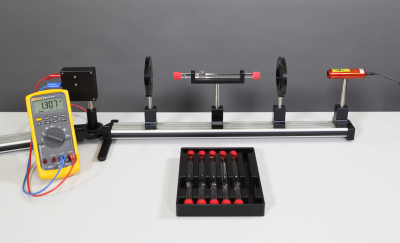
\includegraphics[width=\textwidth]{bilder/Zucker.png}
			\caption{Aufbau des vierten Teilversuches\cite{WWU}}
			\label{fig:Zucker}	
		\end{figure}
		Der Aufbau des vierten Teilversuches ist in Abb. \ref{fig:Zucker} dargestellt.
		Auch hier wird erneut Materie zwischen die Polarisatoren gebracht.
		Dieses Mal handelt es sich um mit Zuckerlösung gefüllte Röhren unterschiedlicher Konzentration.
		Hier sollen die Winkel, an dem zweiten Polarisator, für die unterschiedlichen Konzentration untersucht werden, an denen Minima der Spannung auftreten.
		Daraus lässt sich eine Funktion des Winkels in Abhängigkeit der Konzentration aufstellen und die unbekannte Konzentration der "U"-Röhre über dessen Winkel bestimmt werden.
		
	\subsubsection*{Durchführung}
		
		\begin{figure}[ht]
			\centering
			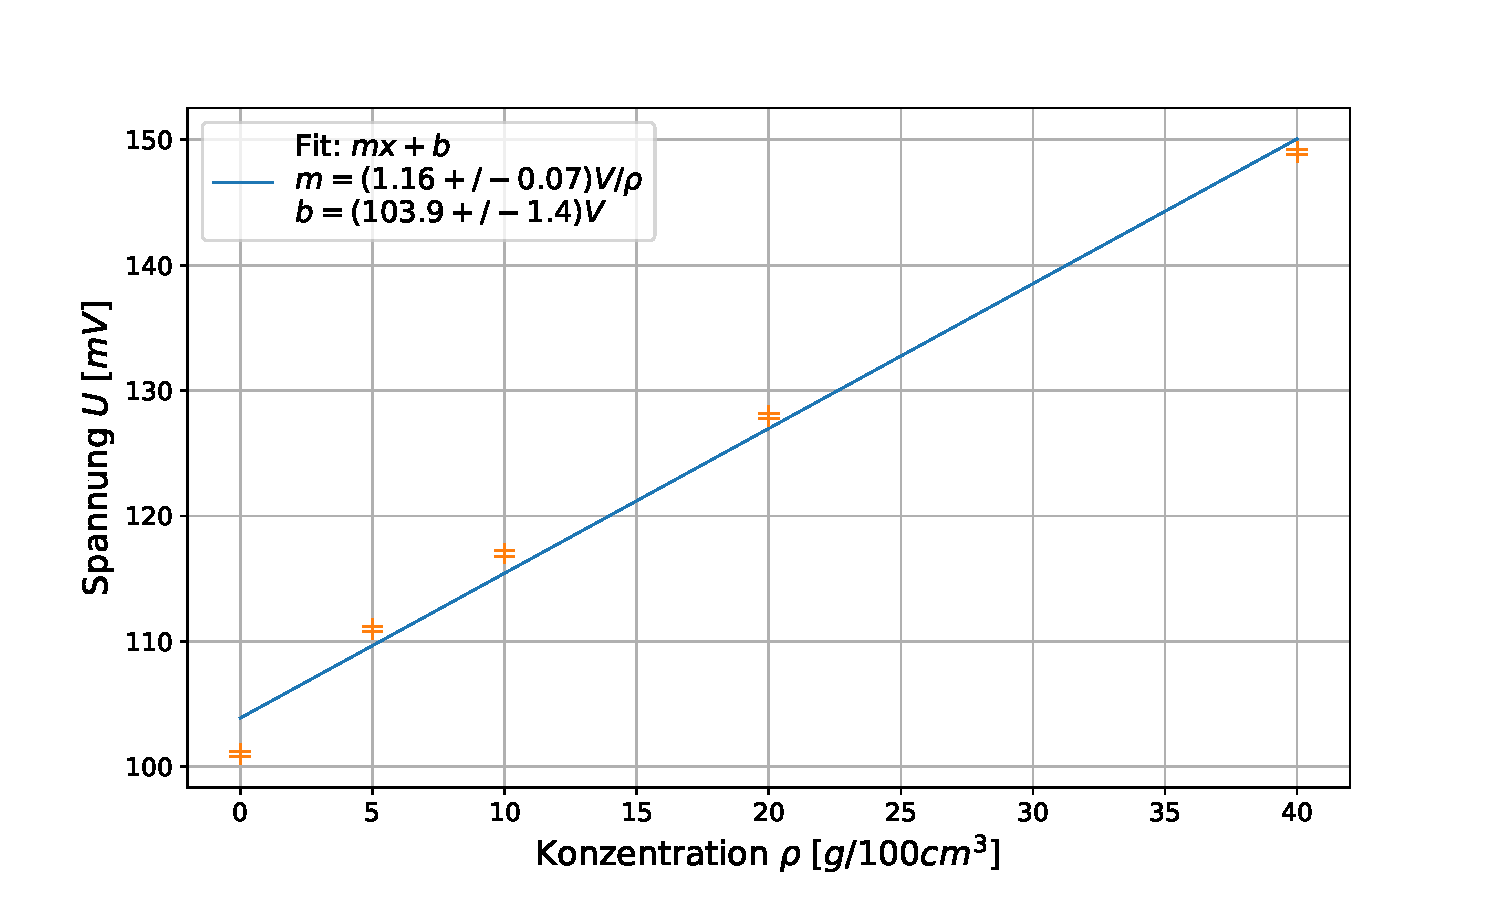
\includegraphics[width=\textwidth]{data/konzentration.pdf}
			\caption{Messpunkte und linearer Fit für die Röhren mit bekannter Zuckerkonzentration}
			\label{fig:ZuckerGerade}	
		\end{figure}
		Für die unterschiedlichen Konzentrationen wurden die Winkel aufgetragen, bei denen das Minimum der Spannung auftrat.
		Bei den Messpunkten ließ sich ein linearer Verlauf beobachten.
		Diese sind in Abb. \ref{fig:ZuckerGerade} aufgeführt.
		Der Winkel der "U"-Röhre belief sich auf \SI{43+-0,4}{\degree}, welcher zwischen den beiden Winkeln für die Röhren mit einer Konzentration von \SI{200}{\gram\per\liter} und \SI{400}{\gram\per\liter} lag.		
	
	\subsubsection*{Datenanalyse}
		
		Die Linearität $\alpha$ zwischen Konzentration und Strahlenversatz setzt sich aus dem spezifischen optischen Drehvermögens $\alpha_s$ mal der Schichtdicke $d$ der Flüssigkeit zusammen.
		In Abb. \ref{fig:ZuckerGerade} ließ sich $\alpha$ durch $m=\SI{1,16+-0,07}{\volt\per\rho}$ beschreiben. % TODO Spannung, Joey?
		Aus dem verwendeten linearen Fit, ließ sich die Konzentration der "U"-Röhre auf $\rho = \SI{252+-20}{\gram\per\liter}$ bestimmen.
	
	\subsubsection*{Diskussion}
	
		Auch an dieser Stelle lässt sich die Erwartung eines linearen Verlaufs, aufgrund der wenigen Messpunkte jedoch nur ungenau, bestätigen.
		Dass der Wert für die Konzentration der "U"-Röhre von $\rho = \SI{252+-20}{\gram\per\liter}$ zwischen \SI{200}{\gram\per\liter} und \SI{400}{\gram\per\liter} lag, stimmt zudem mit der Beobachtung der Winkel überein.
		